\subsection{\textbf{RQ1:} How do practitioners approach merge conflicts?}\label{RQ1}
To understand the perspective of practitioners when encountering a merge conflict, we asked interview participants a series of questions asking them to reflect on situations when they initially face a merge conflict: what kind of information do they seek, how do they approach the resolution of the conflict, and what tools they use. 

We identified nine factors (from card sorting) that practitioners consider when approaching a conflict and to determine its difficulty (see Table~\ref{survey_merge_conflicts}). 

%We then use the results of the interviews to influence the construction of the survey.
We used these nine factors to ask survey participants to rate how each of these factors affected their perceptions of difficulty when approaching a merge conflict
%The survey then asked participants to rate how much each of these 9 factors affected their perceptions of difficulty when approaching a merge conflict. 
The question used a 5-point Likert scale to indicate the degree to which a factor affected conflict difficulty (1 being \textit{Not at all}, 3 being \textit{A moderate amount}, and 5 being \textit{A great deal}).

We received 162 responses and present the aggregated results in Table~\ref{survey_merge_conflicts}.
Here, we discuss further in detail the top 4 factors based on mean scores of the answers (these have a score greater than 3).
These factors can be grouped into \textit{Technical Factors} and \textit{Expertise factor}.

\begin{table*}[!htbp]
\renewcommand{\arraystretch}{1.3}
\caption{Practitioners' Needs for Merge Conflict Resolutions from Survey}
\label{survey_res_diffs}
\centering
\begin{tabularx}{0.87\textwidth}{>{\rowmac}c | >{\rowmac}l | *5{>{\rowmac}c} | *2{>{\rowmac}c}<{\clearrow}}

\toprule
	Need & Description & 1 & 2 & 3 & 4 & 5 & Mean & Median \\
\midrule
	\setrow{\bfseries}N1 & How easy it is to understand the code involved in the merge conflict & 0 & 14 & 25 & 65 & 37 & 3.89 & 4 \\
	\setrow{\bfseries}N2 & Your expertise in the area of code with the merge conflict & 1 & 17 & 38 & 49 & 36 & 3.72 & 4 \\
	\setrow{\bfseries}N3 & The amount of information you have about the conflicting code & 2 & 21 & 38 & 48 & 32 & 3.62 & 4 \\
	\setrow{\bfseries}N4 & How well tools present information in an understandable way & 4 & 24 & 47 & 32 & 34 & 3.48 & 3 \\
	N5 & Changing assumptions within the code & 8 & 27 & 45 & 36 & 25 & 3.30 & 3 \\
	N6 & Complexity of the project structure & 6 & 38 & 39 & 41 & 17 & 3.18 & 3 \\
	N7 & Trustworthiness of tools & 17 & 29 & 39 & 32 & 34 & 3.12 & 3 \\
	N8 & Informativeness of commit messages & 18 & 32 & 30 & 44 & 17 & 3.07 & 3 \\
	N9 & Project culture & 13 & 37 & 43 & 27 & 21 & 3.04 & 3 \\
	N10 & Tool support for examining development history & 16 & 40 & 31 & 32 & 22 & 3.03 & 3 \\
\bottomrule
\end{tabularx}
\end{table*}

\Subsubsection{Technical Factors}\label{artifact-based-factors}
Two of the top four factors refer to perceptions about the complexity of merge conflicts (F1, F3), with the third factor being number of conflicting lines, which can be construed as a specific metric of complexity of the conflict (F4). 
\todo{AS: add cite for FPA}
While practitioners mentioned complexity of the line of code and the file, none mentioned using metrics, such as cyclomatic complexity~\cite{fenton2000quantitative}\cite{mccabe1976complexity} or Function Point Analysis~\cite{...}. Instead, practitioners made educated guesses on the complexity of the code based on their own experience in writing the code or having worked with it. Some of the simple to compute metrics, such as number of conflicting lines of code (F4), number of files involved (F8), atomicity of changesets (F6), and the time they thought it would take to resolve the conflict (F5) were mentioned. The only factor where static analysis tools can help was in identifying the dependencies of the conflicting code (F7).
This indicates that understanding the complexity of the conflicting code is important, but practitioners do not seem to use the metrics that have been proposed by research. While some of the simple proxies for complexity are used, mostly they rely on their own ``judgement" of the complexity of the conflict.
%Researchers have thus far computed complexity of changes in code using proxies such as lines of code changed and numbers of files changed~\cite{khoshgoftaar1990predicting}.
%Other code-centric metrics such as cyclomatic complexity~\cite{fenton2000quantitative}\cite{mccabe1976complexity} and atomicity changes~\cite{khelladi2016ad} can also be used, but require some amount of computation.
%We found that practitioner's perceptions of complexity are just as important in determining how they approach the resolution of a merge conflict.



The perception of the conflict complexity can affect whether a practitioner resolves the conflict immediately (when it is small), or whether they should wait to examine the conflict when further resources can be allocated.
In the interview, P8 commented:
\begin{displayquote}
\textit{``Small is always easy. A 1-line merge conflict is always easier to resolve than a 400-line merge conflict, and can be done now.''}
\end{displayquote}

If a merge conflict is perceived to be large or complex, a practitioner may decide to forgo attempting to resolve it through code manipulation and choose to revert the changes instead~\cite{Guzzi2015}.
This ``nuclear option'' requires practitioners to disrupt the development flow, set aside their current development work, and potentially remove ``good'' code that was not part of the conflict in order to return to a non-conflicting state.
In the interview, P1 describes this process as:
\begin{displayquote}
\textit{``If you have many conflicts involved, many commits involved in the conflict, you should probably throw one of the branches away. Seriously. You cannot combine ...tens of commits conflicting...it's not sane.''}
\end{displayquote}

Further, when integrators are preparing code for production environments they prioritize merge conflicts for code review based upon the perceived difficulty of resolving the affected code.
We find that these decisions rely on humanistic factors as much as they rely on data-driven metrics.
Practitioners may not have the time to compute project-wide complexity metrics, such as those proposed in  literature. Therefore, we need metrics that can be easily calculated by ``lay practitioners" as they face a conflict. 
%are human-aware and take into account the perceived difficulties of merge conflicts.

\Subsubsection{Expertise}\label{knowledge-based-factors}
Our findings show that expertise in the area of conflicting code is one of the top factors in determining the difficulty of a merge conflict (F2). This reiterates the fact that practitioners rely on their own knowledge about the conflicting code base when approaching a conflict. 

Our results indicate that when practitioners feel they don't have the expertise in the conflicting code base, they consider the conflict difficult to merge and seek out more information or help from others. 
P5 illustrated this need for expertise when describing his workflow: 
\begin{displayquote}
	\textit{``A lot of what I work on is\textellipsis in my own little area, so when there is a merge conflict in that area, I will know what to do\textellipsis But if I'm\textellipsis in the [unfamiliar part of project], then I'll\textellipsis get someone else to\textellipsis resolve the merge conflict for me\textellipsis It's someone else's, and I don't want to screw it up.''}
\end{displayquote}



%The importance of the knowledge-based factor indicates that practitioners attribute value to information; the greater knowledge in the conflicting code, the more likely it can be resolved correctly.
%When information is not available, practitioners seek others with expertise to fill this information gap.

%When attempting to resolve a conflict alone, practitioners working in unfamiliar code often feel uncomfortable making decisions during a merge due to lack of familiarity with the code or impacts related to the code change~\cite{CostaSarma}. 
%Situations such as these raise questions relating to which person is best suited to resolve the conflict without introducing a new bug or unintentionally changing code behavior. 

Our findings confirm the need for tools that identify appropriate experts~\cite{CostaSarma} and encourage further research into selection of knowledgeable practitioners for merge conflict resolution.


%We find that expertise, as well as awareness of specific expert knowledge among teams, is an important factor in determining the difficulty of a merge conflict.
%The ability to know who to contact in order to resolve a merge conflict partially explains the drive towards specific integrator and release engineer roles increasing appearing in many software development projects~\cite{adams_release_eng}.

%The results of our survey indicate that \textit{complexity of conflicting lines of code} and \textit{knowledge/expertise in the area of conflicting code} are factors that practitioners find have a direct effect on the perceived difficulty of a merge conflict.
%Although we found consensus across all demographics, the experience level of respondents had an affect on the degree to which they responded affirmatively for these factors (see Table~\ref{survey_merge_conflicts}).
%
%Practitioners with 1-5 years and 6-10 years of experience were only nominally in agreement that merge conflict difficulty is affected by \textit{complexity of conflicting lines of code} (mean: 3.31 and mean: 3.37 respectively) and \textit{knowledge/expertise in the area of conflicting code} (mean: 3.21 and mean: 3.42 respectively).
%As practitioner experiences increases, the level of agreement increases on both of these factors, with practitioners indicating 26+ years experience having the highest consensus (mean: 4.06, std. deviation: 0.77). 
%
%Larger, more complex projects typically require that developers have more experience and a higher degree of knowledge about the systems used in the project.
%As the size of a software project increases, so does the complexity of the underlying code~\cite{banker1993software}\cite{curtis1979third}.
%Therefore, more experienced practitioners are likely to have a broader range of understanding about both \textit{complexity of conflicting lines of code} and \textit{knowledge/expertise in the area of conflicting code} and their affects on merge conflict difficulty.
%
%\begin{figure}[!t]
%\centering
%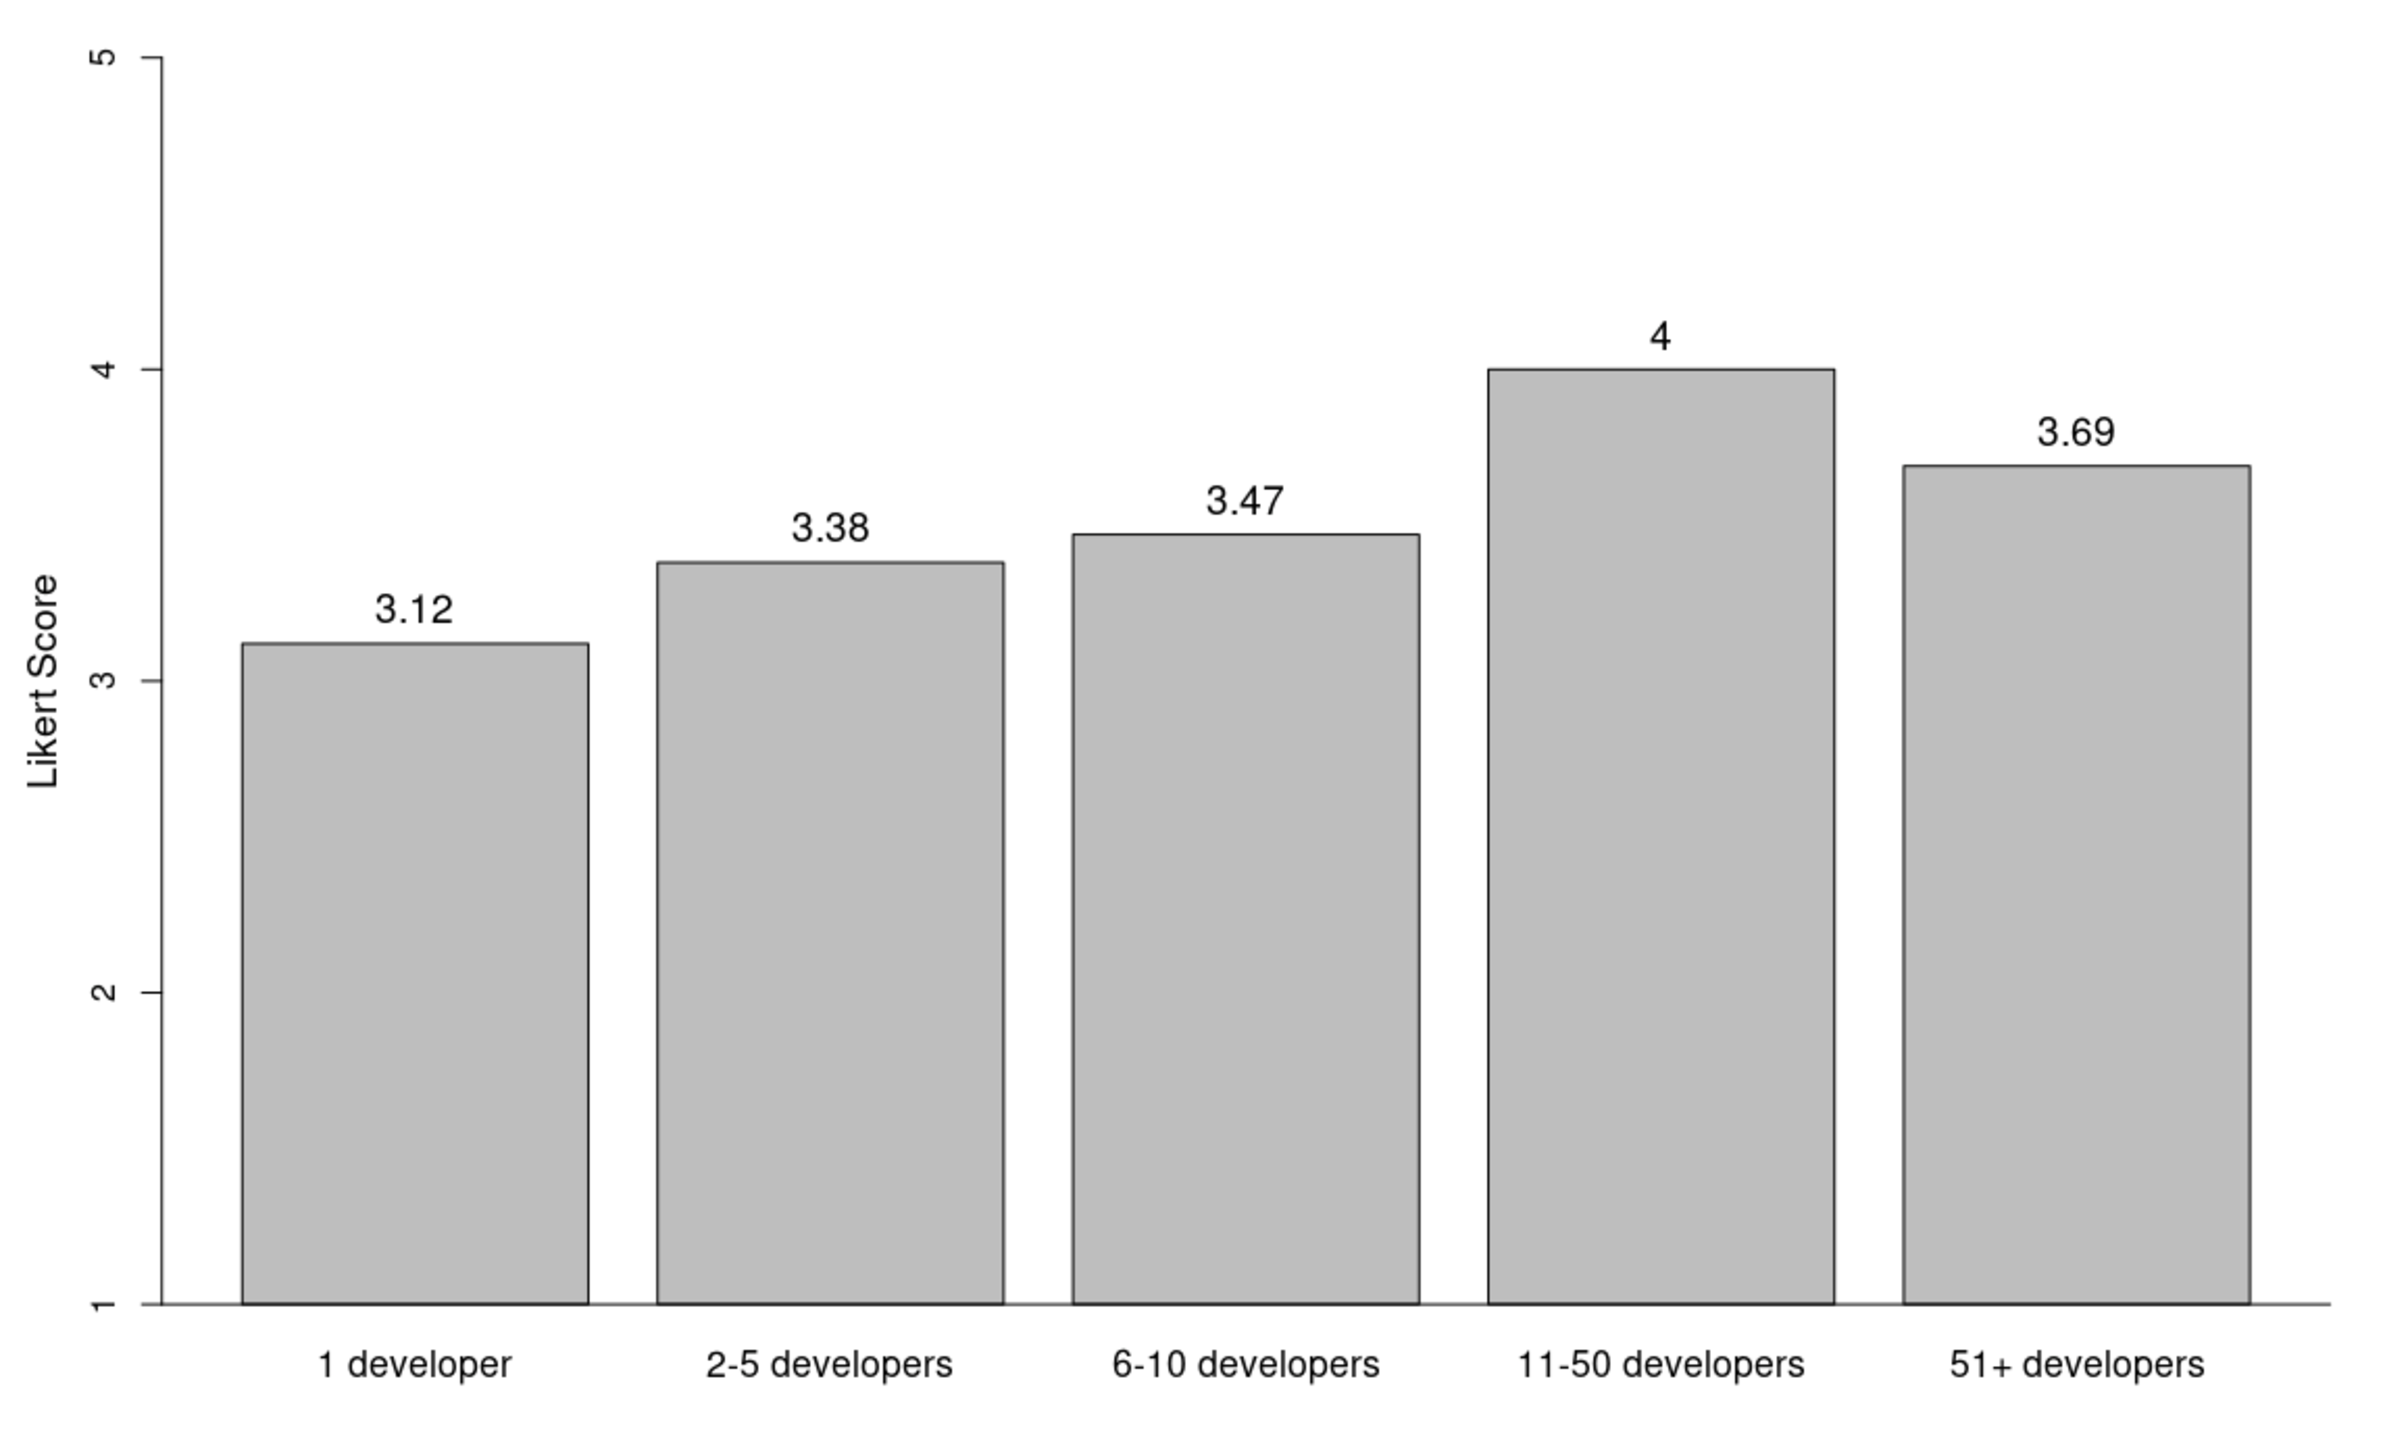
\includegraphics[width=3.4in]{MeanProjectSize.pdf}
%\caption{Mean Likert Score by Project Size for \textit{knowledge/expertise in the area of conflicting code} category of factors that effect the perceived difficulty of merge conflicts.}
%\label{mean_likert_project_size}
%\end{figure}
%
%When analyzing by the size of project that practitioners normally work on, we found that \textit{knowledge/expertise in the area of conflicting code} was increasingly viewed as having an effect on merge conflict difficult as the practitioners' project size increased (see Figure~\ref{mean_likert_project_size}).
%The practitioners that usually work in project sizes of \textit{1 developer}, \textit{2-5 developers}, and \textit{6-10 developers} had relatively neutral responses regarding the effects of \textit{knowledge/expertise in the area of conflicting code} (mean: 3.12, mean: 3.38, and mean: 3.47 respectively).
%However, practitioners that usually work in project sizes of \textit{11-50 developers} and \textit{51+ developers} more positively indicated that \textit{knowledge/expertise in the area of conflicting code} has an effect on the difficulty of merge conflicts (mean: 4.00 and mean: 3.69 respectively).
%
%We also found that practitioners agree that \textit{non-functional changes (whitespace, renaming, etc.)} (mean: 2.16, std. deviation: 1.03) has no effect on the perceived difficulty of a merge conflict.
%Non-functional changes are textual conflicts that can be resolved without consideration of dependencies, performance, or scope.
%Practitioners have less to reason about when resolving merge conflicts that involve only textual conflicts, and therefore are unlikely to perceive \textit{non-functional changes} as affecting the difficulty of merge conflicts.

%Intuitively, we would assume that an increased perception of \textit{knowledge/expertise in the area of conflicting code} as difficulty factor would correlate with a decreased perception of \textit{complexity of conflicting lines of code} as a difficulty factor of merge conflicts.
%This relationship would indicate that a developer's expertise allows them to rationalize about merge conflicts with higher complexity, since they have a higher degree of past knowledge in that area of conflict.
%However, we find a statistical significant correlation between \textit{complexity of conflicting lines of code} and \textit{knowledge/expertise in the area of conflicting code} (Pearson's correlation coefficient: 0.2766, p-value: 0.0003664, 95\% confidence interval: 0.1279 0.4132).
%This suggests that ...

%%%%%%%%%%%%%%%%%%%%%%%%%%%%%%%%%%%%%%%%%%%%%%%%%%%%%%%%%%%%%%%%%

%\subsubsection{Interviews}
%%The interview results suggest that developers approach merge conflicts...
%
%\subsubsection{Survey}
%Our survey suggests that regardless of gender, developer role, experience level, project size, and source distribution model, software practitioners say that the following factors affect the difficulty of a merge conflict most: 
%\begin{itemize}
%\item \textit{Complexity of conflicting lines of code}
%\item \textit{Your knowledge/expertise in area of conflicting code}
%\end{itemize}
%
%Similarly, software practitioners across every measured demographic perceived the following factors to be less important when deciding the difficulty of a merge conflict:
%\begin{itemize}
%\item \textit{Non-functional changes (whitespace, renaming, etc)}
%\item \textit{Number of files in the conflict}
%\end{itemize}
%
%While survey participants did not agree that non-functional changes strongly factor into the difficulty of a merge conflict, it is still worth noting that several interview participants named non-functional changes, such as large refactor or reformatting changes, as a cause for merge conflicts. This suggests that non-functional changes may increase the likelihood of a merge conflict happening, but they do not contribute to the conflict's difficulty.
%
%However, some demographics do view certain difficulties. For instance, open-source developers think that \textit{Atomicity of change sets in the conflict} impacts the difficulty, while closed-source developers and people who split their time evenly think that atomic change sets have no effect on the difficulty. This may be explained by the findings in Rigby et al\cite{OSS_smaller_commits}, which shows that open-source projects tend to review smaller changes than closed-source projects because "The small size lets reviewers focus on the entire change, and the incrementality reduces reviewers’ preparation time and lets them maintain an overall picture of how the change fits into the system." It is possible that our result reflects this difference of culture.
%
%We also found that Project Maintainers say that \textit{Time to resolve a conflict} has an effect, while no other role agrees. This suggests that those in a maintainer role may be more subject to time-related constraints such as maintenance or release schedules. 
%
%\comment{Project Managers say no effect because they focus on project schedules, not conflict resolutions, i.e. they are higher level/abstraction?}
%
%\todo{might be previous work}
%Support and infrastructure roles (System Engineer, Sys Admin, System Architect, DevOps) emphasized that \textit{Dependencies of conflicting code on other components} have more of an effect than other roles did. This might be due to infrastructure systems being maintained in a live environment, or systems that are currently in production use and at risk of real-time dependency failures. 
%
%Developers on projects of size 1 say that \textit{Dependencies of conflicting code on other components}. Because no other project sizes agree with this idea, we hypothesize that this could be due to their high dependence on external code because of the software production limitations of a 1-developer team.
%
%We also found that the group of developers with 21-25 years of experience frequently contradicted general consensus, but it seems more likely that these differences were simply due to the group's small sample size (4).

%We asked participants how much they trust their merging, history exploration, and/or conflict resolution tools, and 57.9\% of participants reported that they trusted these tools either \textit{A Lot} or \textit{Completely}. While this is a majority of developers, this still leaves a significant number of people (42.1\%) who trust their tools \textit{A moderate amount} or \textit{A little}. Though we had the option for \textit{Not at all}, no participants selected this option, presumably because users stop using tools that they do not trust at all. While we found no previous work discussing the threshold for how much users must trust tools for a good tool experience, we postulate that users who cannot trust their tools \textit{A Lot} or \textit{Completely} will avoid relying on such tools too much.